\textbf{Входные параметры:}
 
  Fitness --- массив пригодностей (В отличии от HML\_ProportionalSelection вектор пригодностей должен быть именно вектором пригодностей, то есть все элементы Fitness должны быть больше нуля);
  
 VHML\_N --- размер массива пригодностей.

\textbf{Возвращаемое значение:} 

Номер выбранной пригодности, а, соответственно, номер индивида популяции.

 \textbf{Принцип работы:}

\begin{figure} [h]
  \center
  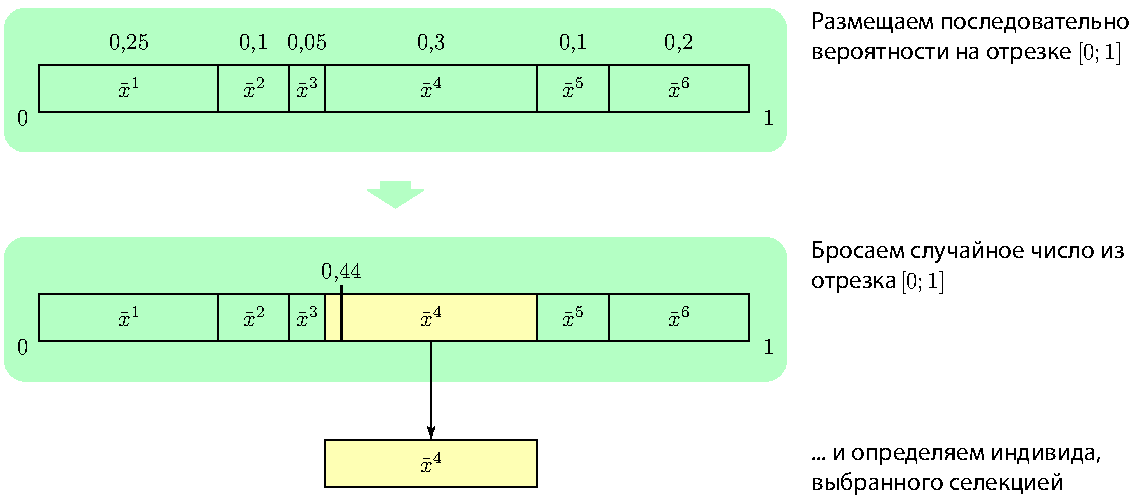
\includegraphics [scale=0.8] {HML_ProportionalSelection_Sheme}
  \caption{Механизм работы пропорциональной селекции} 
  \label{img:HML_ProportionalSelection_Sheme}  
\end{figure}

\textbf{Примечание:}

Данная функция аналогична по действию (результат действия аналогичен):
 
 \begin{enumerate}
\item Связке функций HML\_MakeVectorOfProbabilityForProportionalSelectionV2 и HML\_ProportionalSelectionV2;
\item Функции HML\_ProportionalSelection.
 \end{enumerate}
 
 Различия по временным затратам на выполнение. Эта реализация быстрее, чем HML\_SelectionProportional
 и почти равна связке функций HML\_MakeVectorOfProbabilityForProportionalSelectionV2 и HML\_ProportionalSelectionV2,
 но реализация отличается от формульной записи в угоду более простой записи в программировании, но ей тождественна.
  
\textbf{Примечание:}

Под массивом пригодностей понимается специально преобразованный массив значений целевой функции. Процесс подробно описан в стандарте генетического алгоритма. Смотреть здесь. Но это если Вы используете в алгоритмах оптимизации подобных генетическому. а так, если будете использовать, то учитывайте, что массив пригодностей --- это массив вещественных чисел из отрезка $[0;1]$.

